\documentclass[conference]{IEEEtran}
\IEEEoverridecommandlockouts
% The preceding line is only needed to identify funding in the first footnote.
\usepackage{cite}
\usepackage{amsmath,amssymb,amsfonts}
\usepackage{algorithmic}
\usepackage{graphicx}
\usepackage{textcomp}
\usepackage{xcolor}
\usepackage{url}
\def\BibTeX{{\rm B\kern-.05em{\sc i\kern-.025em b}\kern-.08em
    T\kern-.1667em\lower.7ex\hbox{E}\kern-.125emX}}

\begin{document}

\title{Risk-Aware Distributional Reinforcement Learning\\for 5G-Advanced Handover Decisions}

\author{\IEEEauthorblockN{Gerard Grau Garcia}
\IEEEauthorblockA{gerard.grau.garcia@estudiantat.upc.edu \\
\textit{Dept.\ of Signal Theory and Communications} --- \textit{Universitat Politècnica de Catalunya (UPC)}}}

\maketitle

% =====================================================================
\begin{abstract}
Handover (HO) decisions in 5G-Advanced lower-layer triggered mobility (LTM) must
balance throughput against reliability under fast-varying radio conditions, where
rare but costly events---handover and radio-link failures---dominate the user
experience. We cast LTM HO as a Markov decision process and study distributional
reinforcement learning (QR-DQN) with risk-aware action selection. We report two
separable improvements over scalar DQN. First, the distributional learning target
alone lowers the handover, ping-pong and failure rates at equal reward per
decision. Second, a Conditional-Value-at-Risk (CVaR) policy that acts on the lower
tail of the return distribution drives the failure tails down further; the degree
of risk aversion is a single monotone dial that trades a small amount of reward for
reliability, with a knee at CVaR level $\alpha\approx0.25$. We further show that the
tail is best summarized by a single dedicated quantile: an agent that trains and
acts on one quantile at $\tau=\alpha/2$ attains the lowest failure rates of any
learned agent at the output size and inference cost of scalar DQN. On a
$1{,}000$-trajectory 5G LTM benchmark this risk-aware agent cuts the
handover-failure rate of DQN by $40\%$, improves on a hand-tuned LTM
baseline on every user-facing and safety KPI
while issuing fewer handovers, and improves on a published contextual-bandit
baseline in capacity, reliability and handover failures.
\end{abstract}

\begin{IEEEkeywords}
Distributional reinforcement learning, Quantile regression, Risk-sensitive control, 5G NR, Lower-layer triggered mobility,
Handover optimization.
\end{IEEEkeywords}


% =====================================================================
\section{Introduction}

Fifth-generation (5G) networks densify the radio access with many small, overlapping cells, so a moving user equipment (UE) crosses cell boundaries frequently and must be handed over from one cell---or sector---to another many times during a session.
Each handover (HO) is a brief, risk-laden reconfiguration: chosen well it preserves throughput and reliability; chosen poorly it triggers a handover failure (HOF), a radio-link failure (RLF), or an unnecessary ``ping-pong'' (PP) back to the previous cell.
\emph{Lower-layer triggered mobility} (LTM) is the 5G New Radio mechanism that accelerates these decisions by triggering them from fast L1/L2 measurements rather than slower higher-layer signaling; the price of the extra speed is that the choice of \emph{which} cell/sector to connect to at each measurement opportunity must be made under rapidly varying radio conditions.
That selection is the decision problem we study.

Learning-based HO optimization typically casts cell selection as a heuristic rule or a contextual-bandit / scalar value-learning problem that maximizes an \emph{expected} objective---throughput, or a weighted KPI score---sometimes augmented with reconfigurable intelligent surfaces (RIS) and LMMSE channel prediction to improve the underlying signal quality~\cite{cmab_ho}.
Expected-value objectives are risk-neutral: they optimize the \emph{average} outcome and are indifferent to its dispersion.
Yet in LTM the user experience is dominated not by the average step but by rare, disproportionately costly tail events---handover and radio-link failures. The reward does penalize these events, so a mean-optimal policy is pushed to reduce their \emph{average} frequency; but, optimizing only the expectation, it weighs each rare failure by its small probability and has little leverage to suppress the worst-case tail itself.
This motivates a \emph{risk-aware} formulation that acts on the lower tail of the outcome distribution rather than its mean.

In this paper we approach LTM HO with \emph{distributional} reinforcement learning, which models the full return distribution $Z(x,a)$---for a given radio/mobility state $x$ (per-sector signal measurements, the serving cell and UE kinematics) and handover action $a$ (stay, or switch to a prepared cell)---rather than its mean $Q(x,a)$, and with \emph{risk-aware} action selection based on the Conditional Value at Risk (CVaR) of that distribution.
Intuitively, learning the distribution yields a richer training signal, and acting on its lower tail makes the agent avoid worst-case outcomes instead of merely maximizing the average.
Our contributions are:\begin{itemize}
  \item We formulate LTM HO as a Markov decision process and apply
  Quantile-Regression DQN (QR-DQN) with risk-aware action selection on a
  calibrated 5G LTM simulator (Sections~\ref{sec:model}--\ref{sec:method}).
  \item We show that the distributional learning target alone, acting on the mean,
  already improves the mobility and reliability KPIs over scalar DQN~\cite{dqn} at equal
  reward per decision (Section~\ref{sec:results-dist}).
  \item We cast risk aversion as a single CVaR dial and place its three
  encodings---hard CVaR, spectral (soft-step) reweighting, and a single dedicated
  quantile---on a common reward--reliability frontier, finding a monotone trade
  with a knee near $\alpha=0.25$ rather than an interior optimum
  (Section~\ref{sec:results-risk}).
  \item We characterize \emph{where to spend quantile capacity}: the mean is
  sharpened by adding quantiles, whereas the lower tail is best captured by a
  single dedicated quantile trained and acted on at $\tau=\alpha/2$ (``learn what
  you act on''), which attains the lowest failure rates of any learned agent at the
  cost of scalar DQN (Section~\ref{sec:results-bridge}).
  \item On the 5G LTM benchmark we compare the risk-aware policy against a
  hand-tuned LTM baseline and the contextual
  multi-armed bandit (CMAB) of~\cite{cmab_ho}, improving on both across the
  user-facing and safety KPIs (Section~\ref{sec:results-main}).
\end{itemize}


% =====================================================================
\section{Background and Related Work}
\label{sec:related}

\subsection{LTM and Handover Optimization}
In legacy mobility the network reconfigures a UE's serving cell through
higher-layer (RRC) signaling driven by filtered L3 measurements---robust but slow.
\emph{Lower-layer triggered mobility} (LTM) instead prepares one or more candidate cells in advance and lets a fast L1/L2 measurement event trigger the execution of a pre-configured switch, cutting the interruption time but tightening the decision loop.
The operational cost of a mobility policy is captured by a small set of events: a \emph{handover} (HO) whenever the serving cell changes, a \emph{ping-pong} (PP) when the UE returns to a recently left cell within a short window, a \emph{handover failure} (HOF) when the target
link cannot be established, and a \emph{radio-link failure} (RLF) when the serving link collapses after a sustained run of out-of-sync observations within a time window.
A good policy minimizes failures and ping-pongs while sustaining spectral efficiency.
Prior learning-based work optimizes this trade-off with heuristics and contextual bandits over an expected-KPI objective, optionally stacking RIS and LMMSE channel prediction on top to improve signal quality and target pre-selection~\cite{cmab_ho}; this is the closest prior art to ours.
It is, however, risk-neutral---the gap we address.


\subsection{Distributional Reinforcement Learning}
\label{sec:rel-distrl}
Distributional RL predicts the full distribution of the return rather than its expectation. Instead of modeling the scalar action-value $Q(x,a)$ for each state $x$ and action $a$, the agent models the return as a random variable $Z(x,a)$ that obeys the distributional Bellman equation:

\begin{equation}
Z(x,a) \overset{D}{=} R(x,a) + \gamma\,Z(X',A'),
\label{eq:dist-bellman}
\end{equation}
where $\overset{D}{=}$ denotes equality in distribution, $R(x,a)$ is the reward, $\gamma$ the discount factor, and $(X',A')$ the (random) next state--action pair.
Even when the policy ultimately acts on the mean $\mathbb{E}[Z(x,a)]$, learning the distribution provides a richer per-update signal and consistently improves the resulting policy.
Most practical algorithms approximate the cumulative distribution as a staircase function; representative methods include C51~\cite{c51}, QR-DQN~\cite{qrdqn}, IQN~\cite{iqn} and FQF~\cite{fqf}.
We build on QR-DQN, which parametrizes the distribution by the locations of a fixed set of quantiles.


\subsection{Risk-Sensitive Reinforcement Learning}
\label{sec:rel-risk}
In standard distributional RL the greedy action maximizes $\mathbb{E}[Z(x,a)]$,
approximated as the average of the $N$ predicted quantiles
$\tfrac{1}{N}\sum_{i=1}^{N}\theta_i(x,a)$.
One may instead aggregate the $\theta_i$ under a different criterion to obtain a
risk-sensitive policy. Distributions admit no canonical total order---under
stochastic dominance some pairs are simply incomparable---so any scalar
aggregation imposes one, thereby encoding a particular risk attitude.
A common risk-averse choice replaces the expectation with the Conditional Value
at Risk at level $\alpha$, $\mathrm{CVaR}_\alpha$, the average of the worst
$\alpha$-fraction of outcomes. Here $\alpha$ is a tail \emph{fraction} that is
averaged, not a quantile position: for a uniform return on $[-1,1]$,
$\mathrm{CVaR}_{0.5}$ is the mean of the worse half of the outcomes---the values
in $[-1,0]$, i.e.\ $-0.5$---whereas the median is the single $\tau{=}0.5$
quantile, $0$.
More generally, replacing the uniform average by a non-negative quantile
weighting yields a \emph{spectral} (or distortion) risk measure~\cite{acerbi},
with the expectation and $\mathrm{CVaR}_\alpha$ as the uniform and
lower-tail-uniform special cases; this weighted-quantile family is the design
space for the risk-aware policies we study.
In problems such as LTM HO, risk-aware decision-making is attractive because
avoiding worst-case outcomes (handover or radio-link failures) is more valuable
than maximizing the expected return alone.
CVaR and related risk-sensitive criteria have a long history in reinforcement
learning and operations research~\cite{rockafellar,chow2014,tamar2015};
distributional RL makes them particularly convenient, since the return quantiles
needed to evaluate $\mathrm{CVaR}_\alpha$ are predicted directly by the
distributional Q-value network.

\section{System Model and Problem Formulation}
\label{sec:model}

\subsection{5G LTM Deployment and Simulator}
We evaluate on a calibrated multi-sector 5G deployment of $7$ tri-sector base
stations ($21$ sectors), driven by $1{,}000$ pre-computed UE trajectories of
$300$\,s each whose per-sector channel gains are sampled every $10$\,ms. The
simulator advances at this resolution: at each tick it derives the serving
signal-to-interference-plus-noise ratio (SINR) from the channel gains, transmit
power and inter-cell interference, and maps it through a modulation-and-coding
scheme (MCS) to a spectral efficiency; an SINR below the outage threshold yields
zero rate, and a sustained run of outage ticks escalates to a radio-link failure
(RLF). The radio and mobility constants (Table~\ref{tab:sysparams}) follow the
reference LTM implementation of~\cite{cmab_ho}, and our LTM baseline reproduces
that work's published KPIs.

LTM maintains a small set of \emph{prepared} candidate cells---at most $5$,
selected from the strongest neighbors by an RSRP threshold. In
the standard heuristic a prepared cell is \emph{executed} (the UE is handed over
to it) once its RSRP exceeds the serving cell's by a fixed margin. We keep this
preparation machinery unchanged but replace the execution trigger with the
learned agent: whenever at least one non-serving prepared cell exists, the agent
decides \emph{whether}---and to \emph{which} prepared cell---to hand over. The
decision cadence is therefore \emph{event-driven}, the agent being consulted
once per LTM preparation cycle, at intervals that vary with the radio dynamics.
The agent controls only the \emph{execution} decision---the part of LTM
that trades reliability against signaling overhead---while preparation and the
radio physics remain the reference LTM.

\begin{table}[htbp]
\caption{Key simulator constants (calibrated to the reference LTM implementation).}
\label{tab:sysparams}
\centering
 \begin{tabular}{|l|c|}
\hline
\textbf{Parameter} & \textbf{Value} \\
\hline
Base stations $\times$ sectors      & $7 \times 3 = 21$ \\
UE trajectories                     & $1{,}000$ ($300$\,s each) \\
Simulator step                      & $10$\,ms \\
RL decision cadence                 & event-driven (per LTM cycle) \\
Transmit power                      & $25$\,dBm \\
Noise floor                         & $-101$\,dBm ($-174$\,dBm/Hz $\times\,20$\,MHz) \\
Receiver sensitivity                & $-95$\,dBm \\
Outage (RLF) SINR threshold         & $-3$\,dB \\
Preparation offset                  & $-3$\,dB \\
Max.\ prepared cells                & $5$ \\
Execution offset (LTM trigger)$^{\dagger}$ & $3.0$\,dB \\
\hline
\end{tabular}
{\footnotesize $^{\dagger}$The $+3$\,dB execution offset is the LTM baseline's
hard handover trigger; the RL agent replaces it with a learned, value-based
decision.}
\end{table}

\subsection{MDP Formulation}
\label{sec:mdp}
We model LTM HO as a Markov decision process in which the agent acts only at
handover-decision opportunities. These arise once per LTM cycle and are
unevenly spaced in time; we index the agent's successive decisions by $t$ and
treat each as one step.

\textbf{State.} An $88$-dimensional vector: UE speed $(1)$ and serving-cell
tenure $(1)$, the one-hot serving sector $(21)$, per-sector RSRP $(21)$,
moving-average MCS $(21)$ and moving-average SINR $(21)$, and the UE position
$(x,y)$ $(2)$.

\textbf{Action.} At each decision the agent chooses a target from the action set
$\{\text{serving}\}\cup\{\text{prepared}\}$---at most six entries, since
preparation caps the candidate list at $5$. Choosing the serving cell is a
\emph{stay} (no handover); choosing a non-serving prepared cell executes a
handover to it. Because the agent itself fires the handover, it replaces LTM's
$+3$\,dB execution trigger with the learned value of acting now versus staying,
while preparation and the candidate restriction remain the reference heuristic.

\textbf{Reward.} Each decision is rewarded over the interval until the next
decision by the multiplicative LTM HO reward of~\cite{cmab_ho},
\begin{equation}
R_t = R^{\mathrm{thr}}_t \,\cdot\,
      \frac{\alpha_{\mathrm{HO}}^{\,\mathbb{I}^{\mathrm{HO}}_t}\;
            \alpha_{\mathrm{PP}}^{\,\mathbb{I}^{\mathrm{PP}}_t}\;
            \alpha_{\mathrm{HOF}}^{\,\mathbb{I}^{\mathrm{HOF}}_t}}
           {1 + e^{\,2\,(N^{\mathrm{OOS}}_t - 2)}},
\label{eq:reward}
\end{equation}
where $R^{\mathrm{thr}}_t$ is the throughput term---the serving spectral
efficiency (bps/Hz) \emph{averaged over the decision interval}; the indicators
$\mathbb{I}^{\mathrm{HO}}_t,\mathbb{I}^{\mathrm{PP}}_t,\mathbb{I}^{\mathrm{HOF}}_t\in\{0,1\}$
flag whether a handover, ping-pong or handover failure occurred \emph{anywhere
within} that interval; and
$\alpha_{\mathrm{HO}},\alpha_{\mathrm{PP}},\alpha_{\mathrm{HOF}}\in(0,1]$ are the
corresponding multiplicative penalties (defaults $\alpha_{\mathrm{HOF}}{=}0.1$,
$\alpha_{\mathrm{HO}}{=}0.8$, $\alpha_{\mathrm{PP}}{=}0.9$, so a failure is
penalized far more harshly than a routine handover). The final factor is a
reverse sigmoid of the out-of-sync counter $N^{\mathrm{OOS}}_t$ (the number of
consecutive out-of-sync indications on the serving link): it stays near $1$
while the link is in sync, equals $0.5$ at $N^{\mathrm{OOS}}_t{=}2$, and decays
toward $0$ as the link approaches radio-link failure.
Since the penalty factors lie in $(0,1]$, the reward is the portion of the
attainable throughput $R^{\mathrm{thr}}_t$ that the policy retains after mobility
events and link instability, which the distributional agent models as a random
return.
Because decisions are event-driven, a policy's own choices change how many actions it
faces per episode; we therefore compare policies by their mean reward
\emph{per decision} rather than the episode sum, which would otherwise credit a
policy merely for being consulted more often (Section~\ref{sec:setup}).


% =====================================================================
\section{Method}
\label{sec:method}

\subsection{QR-DQN and the Quantile Loss}
QR-DQN parametrizes $Z(x,a)$ by its inverse CDF at $N$ quantile fractions
$\tau_1,\dots,\tau_N\in[0,1]$, learning
$\theta_i(x,a)\approx F^{-1}_{Z(x,a)}(\tau_i)$.
These $\theta_i(x,a)$ are the
outputs of a neural network: a shared trunk maps the state $x$ to an output
layer (the \emph{head}) that emits the $N$ quantile estimates for every action
$a$, and the network parameters $\phi$ are fit by
minimizing the loss defined below.
Vanilla QR-DQN places these at
the midpoints $\tau_i=(i-\tfrac12)/N$ with uniform weights $w_i=1/N$. The
aggregated value used for action selection,

\begin{equation}
\mathbb{E}[Z(x,a)] = \int_0^1 F^{-1}_{Z(x,a)}(\tau)\,d\tau
\;\approx\; \sum_{i=1}^{N} w_i\,\theta_i(x,a),
\label{eq:expectation}
\end{equation}
is a finite-sample quadrature with weights $w_i\ge 0$, $\sum_i w_i = 1$; the pair
$(\tau_i,w_i)$ defines the \emph{quantile scheme}, and the midpoint choice is the
midpoint Riemann sum for $\int_0^1 F^{-1}(\tau)\,d\tau$. Risk sensitivity is
introduced later (Section~\ref{sec:method-risk}) by altering this aggregation
and, for some variants, the placement of the trained quantiles; the loss below
keeps the same form throughout.

The quantiles are trained with the quantile (pinball) Huber loss. Writing the
Huber function with threshold $\kappa$ as

\begin{equation}
\mathcal{H}_\kappa(u) =
\begin{cases}
\tfrac12 u^2, & |u|\le\kappa,\\[2pt]
\kappa\big(|u|-\tfrac12\kappa\big), & |u|>\kappa,
\end{cases}
\end{equation}
the quantile-Huber penalty at fraction $\tau$ is

\begin{equation}
\rho^\kappa_\tau(u) = \big|\tau - \mathbb{I}\{u<0\}\big|\,
\mathcal{H}_\kappa(u),
\label{eq:pinball}
\end{equation}
The Huber threshold $\kappa$ rounds the kink of the plain pinball
(absolute-value) loss into a quadratic region near zero, giving bounded,
continuous gradients that are robust to the large bootstrapped errors common
early in training~\cite{qrdqn}. The asymmetric prefactor
$|\tau-\mathbb{I}\{u<0\}|$ is what makes this \emph{quantile} regression rather
than ordinary regression: it penalizes errors asymmetrically---weight $\tau$ on
one side of zero and $1-\tau$ on the other---so the per-quantile loss is minimized
when $\theta_i$ sits at the $\tau_i$-quantile of its target rather than at the
mean.
The per-transition loss sums the pairwise temporal-difference errors between
each of the $N$ \emph{predicted} quantiles (the online network's current outputs)
and each of the $N$ \emph{target} quantiles
$y_j = r + \gamma\,\theta_j\!\big(x',a^\star\big)$ (bootstrapped from a frozen
target network),

\begin{equation}
\mathcal{L}(x,a) = \frac{1}{N}\sum_{i=1}^{N}\sum_{j=1}^{N}
   \rho^{\kappa}_{\tau_i}\!\big(y_j - \theta_i(x,a)\big),
\label{eq:qr-loss}
\end{equation}
with $a^\star$ the greedy action under the aggregated value~\eqref{eq:expectation}.
Equation~\eqref{eq:qr-loss} is best read as a sum of independent per-quantile
regressions. Ideally each prediction $\theta_i(x,a)$ would be fit to its
\emph{expected} quantile-Huber loss against the bootstrapped target
$Y = r + \gamma Z(x',a^\star)$ (i.e.\ minimizing
$\mathbb{E}\!\big[\rho^\kappa_{\tau_i}(Y-\theta_i(x,a))\big]$, whose minimizer is
the $\tau_i$-quantile of $Y$). Since $Y$ is unavailable in closed form, we
represent it by its own $N$ predicted quantiles $\{y_j\}$ and average their losses
(the $\tfrac1N$ factor). Every predicted quantile is therefore regressed
against \emph{all} $N$ targets---the whole bootstrapped return distribution---rather
than a single scalar value, and it is this distribution-to-distribution regression
that drives the network to recover the shape of $Z(x,a)$.

\subsection{Risk-Aware Quantile Aggregation}
\label{sec:method-risk}
The quantile loss~\eqref{eq:qr-loss} fixes how the return distribution is
learned but leaves the aggregation~\eqref{eq:expectation} free. A risk-sensitive
policy keeps the same network and replaces the uniform average by a non-negative
weighting
\begin{equation}
Q_\omega(x,a) = \sum_{i=1}^{N}\omega_i\,\theta_i(x,a),
\qquad \omega_i\ge 0,\ \textstyle\sum_i\omega_i = 1,
\label{eq:risk-agg}
\end{equation}
acting greedily on $Q_\omega$ (so $\omega$ also selects $a^\star$ in
\eqref{eq:qr-loss}). When $\omega_i$ is non-increasing in $\tau_i$ this is a
\emph{spectral} (distortion) risk measure (Section~\ref{sec:rel-risk}), with the
expectation as its uniform special case. We make the policy tail-averse in two
ways: by \emph{re-weighting} the quantiles of a faithfully trained distribution
(the hard-CVaR and soft-step policies below, with the mean as the risk-neutral
baseline), which leaves~\eqref{eq:qr-loss} untouched and therefore adds nothing at
inference; or by \emph{re-placing} the trained quantiles onto the tail (truncation
and the single-quantile policy), which instead concentrates network capacity where
the policy acts.

\textbf{Risk-neutral (mean).} Setting $\omega_i=w_i=1/N$ recovers the
expectation; this is our risk-neutral (RN) agent, the direct distributional
counterpart of DQN. It carries no tail preference but still benefits from the
richer per-update signal of~\eqref{eq:qr-loss}.

\textbf{Hard CVaR.} The standard risk-averse criterion is the conditional value
at risk at level $\alpha$, the mean of the worst $\alpha$-fraction of returns---on
the midpoint grid, a uniform average over the lowest $k=\lceil\alpha N\rceil$ of
the $N$ quantiles (ordered by increasing $\tau_i$):
\begin{equation}
\omega_i^{\mathrm{CVaR}} = \frac{\mathbb{I}\{i\le k\}}{k},
\label{eq:cvar}
\end{equation}
a hard $0/1$ step at the $k$-th quantile. The upper $N-k$ quantiles are
trained but never consulted at decision time.

\textbf{Soft-step (spectral).} Hard CVaR is the limit of a one-parameter family
that relaxes the step to two finite levels: the lowest $k$ quantiles receive
$r\ge 1$ times the weight of the rest,
\begin{equation}
\omega_i(r) =
\frac{r\,\mathbb{I}\{i\le k\} + \mathbb{I}\{i>k\}}{r\,k + (N-k)} .
\label{eq:softstep}
\end{equation}
Here $r{=}1$ gives back the mean (RN) and $r\to\infty$ recovers hard
CVaR$_\alpha$~\eqref{eq:cvar}, with intermediate $r$ interpolating a graded tail
emphasis. The positions stay uniform---all $N$ quantiles remain active and
faithfully trained---so risk lives entirely in the weights, and every member is a
valid spectral measure. This realizes the weighted-quantile design space
anticipated in Section~\ref{sec:rel-risk}.

\textbf{Truncated CVaR.} Equation~\eqref{eq:cvar} wastes capacity: the head
predicts $N$ quantiles but only the lowest $k$ enter the decision. The truncated
variant trains \emph{only} $k$ quantiles, placed uniformly
in $[0,\alpha]$; their plain mean equals CVaR$_\alpha$ exactly under the midpoint
rule. This realizes the same risk policy with a smaller head and a tail-only
loss. Concentrating capacity on the consulted region might be expected to sharpen
the estimate; Section~\ref{sec:results-trunc} shows instead that the full and
truncated CVaR policies are statistically indistinguishable on reward per decision
and tail KPIs---truncation buys lower cost and faster training, not a better
policy.

\textbf{Single dedicated quantile (RA-1q).} Taken to its extreme, truncation
keeps a single quantile ($k{=}1$) at $\tau=\alpha/2$---the center of the tail
lobe---and selects on it directly, a VaR-style point criterion. RA-1q learns and
acts on exactly one return statistic, matching the output dimension and inference
cost of scalar DQN. The link is sharpest at the risk-neutral end: with
$N{=}1,\,\tau{=}0.5$ the asymmetric weight $|\tau-\mathbb{I}\{u<0\}|$
in~\eqref{eq:qr-loss} becomes constant ($\tfrac12$) and the loss reduces to a
symmetric Huber regression onto a single robust value (the median in the
un-Huberized limit)---the distributional counterpart of plain value learning. DQN
and RA-1q are therefore two ends of a single-quantile family separated only by the
acted fraction $\tau$ ($0.5$ vs.\ $\alpha/2$). This ``learn what you act on''
design is tested in Section~\ref{sec:results-bridge} against both spreading
capacity over a tail lobe (truncated and full CVaR) and its converse---learning
the full distribution but acting on only its $\tau{=}\alpha/2$ quantile.
Section~\ref{sec:results-risk} places these knobs---hard CVaR, soft-step weights,
and the single dedicated quantile---on a common risk--reliability frontier.


% =====================================================================
\section{Experimental Setup}
\label{sec:setup}

\subsection{Evaluation Protocol and Metrics}
All agents are trained and evaluated on the same $1{,}000$ pre-computed UE
trajectories ($300$\,s each, $10$\,ms simulation resolution), with the agent
consulted at the event-driven handover-decision opportunities of
Section~\ref{sec:mdp}. We deliberately use the full trajectory set for both
training and final evaluation rather than a held-out split: the channel-gain
dataset is fixed and the policy never observes future returns, so the relevant
question is how well each agent exploits the available propagation environment,
not generalization to unseen geometry. Each final model is trained for $2{,}000$
episodes across $5$ random seeds; the comparative studies in
Section~\ref{sec:results} use a lighter $1{,}000$-episode, $3$-seed setting. After
training, we evaluate every agent with frozen weights and greedy action selection
($\epsilon{=}0$), replaying all $1{,}000$ UE trajectories, and report the
cross-seed mean $\pm$ standard deviation throughout. The full implementation
(simulator, agents and evaluation scripts) is publicly available~\cite{code}.

Following Section~\ref{sec:mdp}, we report the mean \emph{reward per decision}---the
episode reward divided by the number of decisions taken---as the primary scalar
objective, since the episode sum otherwise grows simply with the number of
decisions a policy triggers. Alongside it we track the eight physical KPIs
of~\cite{cmab_ho}: handover rate (HO/min), handover-failure rate (HOF/min),
ping-pong rate (PP/min), radio-link-failure rate (RLF/min), spectral efficiency /
capacity (bps/Hz), link reliability (\%), cell preparations (/min) and resource
reservation (\%).

\subsection{Models and Hyperparameters}
\label{sec:models}

We compare four learned agents that share an identical two-layer MLP trunk
($256\times256$) and the same observation, action and reward definitions, so that
differences trace to the \emph{learning target} and the \emph{risk rule} rather
than to trunk capacity or input. They differ only in the output head and how it
is read for action selection (Section~\ref{sec:method-risk}):
\begin{enumerate}
    \item \textbf{DQN}---scalar value learning; greedy $\arg\max_a Q(x,a)$.
    \item \textbf{RN}---risk-neutral QR-DQN; an $N{=}25$ midpoint head read by the
    mean policy $\mathbb{E}[Z(x,a)]$.
    \item \textbf{Soft-step}---the \emph{same} $N{=}25$ head, read instead through
    the soft-step spectral weighting~\eqref{eq:softstep} at $\alpha{=}0.25$ and
    ratio $r{=}2$ (all $25$ quantiles re-weighted, none discarded).
    \item \textbf{RA-1q}---a single dedicated quantile ($k{=}1$) at
    $\tau{=}\alpha/2$ ($\alpha{=}0.25$), matching the scalar head size and
    inference cost of DQN.
\end{enumerate}
These are benchmarked against two references: our own hand-tuned LTM baseline and
the contextual-bandit (CMAB) policy of~\cite{cmab_ho}. We additionally train full- and truncated-CVaR agents,
soft-step agents at several ratios $r$, and single-quantile agents
(Section~\ref{sec:results}), each differing only in the aggregation or trained
grid of Section~\ref{sec:method-risk}.

All agents bootstrap from a frozen \emph{target network} whose parameters
$\phi^{-}$ track the online parameters $\phi$ by a soft update,
$\phi^{-}\!\leftarrow(1{-}\tau)\,\phi^{-}+\tau\,\phi$ with $\tau{=}0.01$, rather
than a periodic hard copy; the greedy next action and its quantiles are both read
from this target network.
Soft and hard updates are within cross-seed noise here, so we fix the soft scheme
for all agents. The remaining hyperparameters (Table~\ref{tab:hparams}) follow
coarse grid searches and the prior work~\cite{cmab_ho}, with one gradient update
every eight environment steps for training speed; network width saturates at
$256\times256$, and $n$-step returns, gradient clipping and optimizer-$\epsilon$
variants gave no improvement.
The Huber threshold $\kappa{=}0.25$ was selected
from a coarse sweep over $\{0.25,0.5,1,2\}$; smaller $\kappa$ gave marginally
higher reward and lower failure rates, and we fix $\kappa{=}0.25$ throughout.

\begin{table}[htbp]
\caption{Shared training hyperparameters. The quantile count applies to RN and
soft-step; RA-1q uses a single quantile ($k{=}1$), and $\kappa$ applies to all
three QR-DQN agents. DQN is a scalar value learner; each agent's risk rule (mean,
soft-step, or single quantile) is given in the agent list of
Section~\ref{sec:models}.}
\label{tab:hparams}
\centering
\begin{tabular}{|l|c|}
\hline
\textbf{Hyperparameter} & \textbf{Value} \\
\hline
Hidden layers       & $256\times256$ \\
Optimizer           & Adam \\
Learning rate       & $10^{-4}$ \\
Discount $\gamma$   & $0.9$ \\
Replay buffer       & $10^{5}$ \\
Batch size          & $256$ \\
Train frequency     & $8$ \\
Target update       & soft, $\tau{=}0.01$ \\
$\epsilon$ schedule & $1.0 \to 0.05$ (geom., $\times0.995/$ep) \\
\hline
Quantiles $N$ (RN, soft-step) & $25$, midpoint \\
Huber $\kappa$ (QR-DQN)       & $0.25$ \\
\hline
\end{tabular}
\end{table}

% =====================================================================
\section{Results on the LTM Handover Task}
\label{sec:results}

\subsection{Distributional Learning on the Handover Task}
\label{sec:results-dist}
We first establish how the two learning agents behave on the handover task before
turning to risk. Scalar DQN and risk-neutral QR-DQN (RN) are trained on the full
set of $1{,}000$ trajectories for $2{,}000$ episodes and evaluated, with results
averaged over five seeds. The two differ only in the output layer: DQN regresses a single
scalar value, whereas RN predicts a full distributional head
(Section~\ref{sec:method}), here $25$ quantiles, and acts on its mean.
Table~\ref{tab:dist} reports both, alongside a single-quantile RN that isolates the
effect of the distributional representation.

\textbf{Distributional learning versus the scalar baseline.}
DQN and RN earn the same reward per decision, yet RN improves on
every other axis: it lowers the handover, ping-pong, and handover-failure rates,
raises capacity and link reliability, and leaves resource use essentially
unchanged (Table~\ref{tab:dist}). For scale, a uniform-random execution
policy---choosing uniformly among the serving and prepared cells, evaluated under
the same protocol---earns only $1.93$ reward per decision and the LTM heuristic
$3.544$ (Section~\ref{sec:results-main}); both learned agents therefore sit near
the achievable ceiling and separate on the mobility and reliability KPIs rather
than on reward itself. Learning the return distribution and acting on
its mean improves the scalar baseline at equal reward.

\textbf{Quantile count for the mean.}
The improvement comes from the full
distribution, not from the quantile loss alone. A risk-neutral head reduced to a
single quantile at $\tau=0.5$ reproduces DQN almost exactly across every metric
(Table~\ref{tab:dist}, middle column): as Section~\ref{sec:method-risk} notes, a
lone median quantile trained under the Huber loss recovers essentially the same
robust value that DQN learns on these near-symmetric returns. The reliability gain
grows as further quantiles populate the head, with the largest step in the first
few and diminishing returns afterward: sweeping $N$ at the study setting, the
handover-failure rate falls from $0.64$/min at $N{=}1$ to $0.55$/min by $N{=}3$ and
eases further to $0.50$/min by $N{=}25$ (handover rate $6.0$, $5.3$, $5.0$/min),
while the reward per decision stays flat (${\approx}3.66$). The $N{=}25$
head we carry throughout (Table~\ref{tab:dist}, right column) is therefore also the
best-performing mean policy, and it supplies the finer tail grid that the CVaR and
soft-step risk studies act on ($k=\lceil\alpha N\rceil$ tail quantiles,
Section~\ref{sec:results-risk}). The quantiles'
\emph{placement}, by contrast, is immaterial:
replacing the midpoint grid with Gauss--Legendre, trapezoidal, Simpson, or
Beta-warped positions leaves the reward per decision within cross-seed noise
(between $3.654$ and $3.663$), so we keep the simple midpoint grid throughout.

\begin{table}[htbp]
\caption{Distributional learning ($2{,}000$ episodes, five seeds). The three
columns isolate the source of the gain: scalar DQN; a distributional head
collapsed to one median quantile ($N{=}1$), which reproduces DQN; and the full
$25$-quantile head---the RN agent used throughout the paper---which lowers the
handover, ping-pong, and failure rates at equal reward. Bold marks the best value
in each row.}
\label{tab:dist}
\centering
\begin{tabular}{|l|c|c|c|}
\hline
\textbf{KPI} & \textbf{DQN} & \textbf{RN ($N{=}1$)} & \textbf{RN ($N{=}25$)} \\
\hline
Reward/decision $\uparrow$          & $3.667{\pm}0.006$ & $\mathbf{3.669{\pm}0.003}$ & $3.663{\pm}0.011$ \\
Capacity (bps/Hz) $\uparrow$        & $4.062$ & $\mathbf{4.072}$ & $4.068$ \\
Reliability (\%) $\uparrow$         & $97.00$ & $97.02$ & $\mathbf{97.07}$ \\
HO/min $\downarrow$                 & $5.63$  & $5.63$  & $\mathbf{5.12}$  \\
PP/min $\downarrow$                 & $1.065$ & $1.079$ & $\mathbf{0.857}$ \\
HOF/min $\downarrow$                & $0.667$ & $0.648$ & $\mathbf{0.551}$ \\
RLF/min $\downarrow$                & $0.047$ & $0.048$ & $\mathbf{0.046}$ \\
Prep/min $\downarrow$               & $28.1$  & $\mathbf{27.6}$  & $27.7$  \\
Res.\ reserv. (\%) $\downarrow$ & $8.85$  & $\mathbf{8.74}$  & $8.91$  \\
\hline
\end{tabular}
\end{table}

\subsection{A Controllable Risk Dial}
\label{sec:results-risk}
Having shown that the distributional representation helps, we now make the policy
risk-averse and ask how the degree of risk-aversion trades against performance.
The CVaR level $\alpha$ is a single dial: $\alpha=1$ recovers the risk-neutral
mean, and smaller $\alpha$ focuses the policy on the lower tail of the return
distribution. We sweep it over $1{,}000$ episodes and three seeds on the $N{=}25$
midpoint head (hard CVaR averaging the lowest $k=\lceil\alpha N\rceil$ quantiles),
and defer how the tail estimate should be \emph{built} to
Section~\ref{sec:results-bridge}.

\textbf{Risk trades monotonically against reward.} Table~\ref{tab:alpha} dials
$\alpha$ from mild ($0.5$) to aggressive ($0.1$). As $\alpha$ decreases the policy
grows more conservative: it hands over less and fails less, while giving up a
little reward, capacity, and link reliability. The trade is monotone and has no
interior optimum---there is no single ``best'' risk level, only a controllable
exchange of reward for reliability. The reward cost is mild while the failure
reduction levels off, leaving a clear knee near $\alpha=0.25$ (also visible in the
frontier of Fig.~\ref{fig:frontier}), which we adopt.

\textbf{The risk--reliability frontier.} The three risk encodings of
Section~\ref{sec:method-risk}---averaging the lower tail (hard CVaR), reweighting a
faithfully trained grid (soft-step), and committing to one dedicated
quantile---can all be placed on a single risk--reliability frontier
(Fig.~\ref{fig:frontier}). Soft-step is its continuous member~\eqref{eq:softstep}: at ratio $r=1$ it is
the risk-neutral mean, and as $r$ grows it shifts weight onto the tail and
approaches hard CVaR, the reward per decision moving from $3.655$ at $r=2$ to
$3.606$ at $r=100$, toward the hard-CVaR value of $3.598$.
We adopt $r=2$ for the headline Soft-step agent: it captures most of the reliability gain at
the favorable, low-curvature end of the frontier, whereas larger $r$ pays
increasing reward for diminishing returns.
The single dedicated
quantile lies on the most favorable edge of the frontier, delivering more reward at
any failure level than the averaging or reweighting schemes; we examine why in
Section~\ref{sec:results-bridge}.

\begin{table}[htbp]
\caption{The hard-CVaR risk dial on the $N{=}25$ head ($1{,}000$ episodes, three seeds), from mild
($\alpha=0.5$) to aggressive ($\alpha=0.1$). Greater risk-aversion lowers the
handover and failure rates at a modest cost in reward, capacity, and link
reliability; the trade is monotone, with a knee near $\alpha=0.25$. Bold marks the
best value in each row.}
\label{tab:alpha}
\centering
\begin{tabular}{|l|c|c|c|}
\hline
\textbf{KPI} & $\alpha{=}0.5$ & $\alpha{=}0.25$ & $\alpha{=}0.1$ \\
\hline
Reward/decision $\uparrow$          & $\mathbf{3.613{\pm}0.016}$ & $3.598{\pm}0.003$ & $3.542{\pm}0.014$ \\
Capacity (bps/Hz) $\uparrow$        & $\mathbf{4.048}$ & $4.019$ & $3.974$ \\
Reliability (\%) $\uparrow$         & $\mathbf{97.00}$ & $96.90$ & $96.71$ \\
HO/min $\downarrow$                 & $4.76$  & $4.33$  & $\mathbf{4.17}$  \\
PP/min $\downarrow$                 & $0.826$ & $0.627$ & $\mathbf{0.498}$ \\
HOF/min $\downarrow$                & $0.442$ & $0.367$ & $\mathbf{0.353}$ \\
RLF/min $\downarrow$                & $0.045$ & $\mathbf{0.043}$ & $0.043$ \\
Prep/min $\downarrow$               & $27.6$  & $26.0$  & $\mathbf{25.9}$  \\
Res.\ reserv. (\%) $\downarrow$ & $9.3$   & $\mathbf{9.3}$   & $9.4$   \\
\hline
\end{tabular}
\end{table}

\begin{figure}[htbp]
\setlength{\abovecaptionskip}{4pt}   % space between image and caption
\setlength{\belowcaptionskip}{0pt}   % space after caption
\centering

\includegraphics[width=\columnwidth]{risk_frontier.png}
\caption{Risk--reliability frontier ($1{,}000$ episodes, three seeds): reward per
decision against the handover-failure rate for the three risk encodings, with the
risk-neutral agent (RN) as the least risk-averse anchor. The single dedicated
quantile (orange) is the efficient frontier---more reward at any failure
level---with its knee at $\alpha=0.25$; soft-step interpolates continuously between
RN and hard CVaR. Upper-left is better.}
\label{fig:frontier}
\end{figure}


\subsection{Where to Spend Quantile Capacity}
\label{sec:results-bridge}
Section~\ref{sec:results-dist} showed that the \emph{mean} is sharpened by adding
more quantiles, with diminishing returns. The risk estimate behaves oppositely: the lower
tail is best summarized by very few quantiles, and in the limit by a single
dedicated one. The studies below use $1{,}000$ episodes and three seeds; the
headline single-quantile agent is also reported at the final
$2{,}000$-episode, five-seed setting.

\textbf{Quantile count for the tail.} Holding the risk level at $\alpha=0.25$ and
averaging the lowest $k$ quantiles (ordered by $\tau$) into the CVaR estimate, the reward per decision
falls steadily as $k$ grows---from $3.634$ at $k=1$ to $3.555$ at $k=25$---while
the failure rate barely moves. Packing the tail more densely does not help either:
at $\alpha=0.4$ a densely truncated head ($3.587$) is worse than a plain one
($3.619$). Where the mean was sharpened by more quantiles, the tail estimate is
only diluted by them.

\textbf{The single dedicated quantile.} The limit $k=1$---one quantile trained and
acted on at $\tau=\alpha/2$ (RA-1q)---is the most efficient point of the study. At
the final setting it attains the lowest failure rates of any learned agent
(HOF $0.399$/min, against DQN's $0.667$; Table~\ref{tab:final}) while matching the
output size and inference cost of scalar DQN, and it trains fastest of all
($76$\,min, versus $87$ for DQN and $141$ for the $25$-quantile RN). Committing the
network's one statistic to the quantile the policy actually consults---``learn what
you act on''---is both the cheapest and the most reliable design.

\textbf{Training the acted quantile.} Acting on a single tail quantile is not
enough on its own; that quantile must also be the one trained. The converse
design---learning the full $25$-quantile distribution but selecting on a single
$\tau=\alpha/2$ quantile---ties RA-1q on reward yet leaves the failure rate
markedly higher (HOF $0.42$--$0.48$ versus $0.374$ in the $1{,}000$-episode studies), while
fitting $25$ quantiles instead of one costs substantially more to train.
Concentrating the loss on the single acted quantile is what sharpens the tail.

\textbf{Full versus truncated heads.}\label{sec:results-trunc} The CVaR policy
itself can be realized two ways: a full $N=25$ head whose lowest
$k=\lceil\alpha N\rceil$ quantiles are averaged, or a truncated head that trains
only those $k$ over $[0,\alpha]$. The two are statistically indistinguishable on
reward per decision and tail KPIs (at $\alpha=0.4$, $3.628$ versus $3.619$);
truncation merely trains faster with a smaller head ($65$\,min versus $79$\,min). It is
an efficiency option, not a better estimator.

\subsection{Comparison with the LTM Heuristic and Contextual Bandits}
\label{sec:results-main}
Table~\ref{tab:final} and Fig.~\ref{fig:bars} report the four learned agents at the final
$2{,}000$-episode, five-seed setting against two references: our hand-tuned LTM
baseline, run in the same simulator and therefore directly comparable, and the
contextual multi-armed bandit (CMAB) of~\cite{cmab_ho}, whose published figures
come from a different simulator and are indicative only (Table~\ref{tab:final},
footnote).

\textbf{Versus the LTM heuristic.} Every learned agent improves on the heuristic
across the user-facing and safety KPIs, and the risk-aware RA-1q does so by the
widest margin: relative to LTM it raises capacity by $7.8\%$ ($4.044$ versus
$3.753$\,bps/Hz) and link reliability by $1.7$ points ($96.94\%$ versus
$95.25\%$), and it cuts the handover-failure rate by $65\%$ ($0.399$ versus
$1.151$/min), the ping-pong rate by $82\%$ ($0.656$ versus $3.625$), and the
radio-link-failure rate by $31\%$ ($0.045$ versus $0.065$).
It also earns more reward per decision than the heuristic ($3.641$ versus
$3.544$), so the advantage holds on the training objective itself.

\textbf{Signaling frugality.} The learned policies are also less active than either
reference, not more. In the event-driven setting they issue far fewer
handovers---$4.6$ to $5.6$ per minute, against $11.3$ for LTM and $8.0$ for
CMAB---and correspondingly fewer ping-pongs. The distributional agents thus achieve
their reliability and throughput gains while \emph{reducing} control-plane
mobility, not by trading signaling for reliability.

\textbf{The resource-reservation trade-off.} The one metric on which the
heuristics lead is resource reservation: the learned agents hold more cells
reserved ($8.8$ to $9.0\%$, versus $6.4\%$ for LTM and $6.8\%$ for CMAB). Keeping
more candidates ready is the cost they pay for their lower failure rates;
preparation rates, by contrast, are comparable across all agents ($24$ to
$28$/min).

\textbf{Relation to contextual bandits.} The CMAB of~\cite{cmab_ho} addresses
the \emph{same} decision as our agent: at each opportunity it selects the handover
target among the candidate cells from contextual features, trained on the
\emph{same} multiplicative reward~\eqref{eq:reward}. It is therefore a direct
alternative to our policy, not a complementary mechanism. The two differ in
\emph{how} the decision is learned: CMAB is a contextual bandit that treats each
decision in isolation---assuming the chosen action does not affect future
context---and optimizes the expected reward, whereas our agent is a sequential,
bootstrapped value learner that additionally acts on the lower tail of the return
distribution. On the user-facing quality KPIs the risk-aware agent improves on the
reported CMAB figures (capacity $4.044$ versus $3.68$, reliability $96.94\%$ versus
$94.0\%$, handover-failure rate $0.399$ versus $0.97$), subject to the
cross-simulator caveat above.

\begin{table*}[t]
\caption{Final performance on the LTM handover task. For the learned agents, the
reward per decision is the cross-seed mean $\pm$ standard deviation over
$2{,}000$ episodes and five seeds (standard deviation across seeds, not a
confidence interval; each seed is evaluated on all $1{,}000$ trajectories).
\textbf{LTM}: our hand-tuned baseline. \textbf{CMAB}$^{*}$: the contextual bandits
of~\cite{cmab_ho}. \textbf{DQN}: scalar baseline. \textbf{RN}: risk-neutral QR-DQN
($N{=}25$). \textbf{Soft-step}: spectral reweighting ($\alpha{=}0.25$, $r{=}2$).
\textbf{RA-1q}: single dedicated quantile ($\alpha{=}0.25$). The LTM reward per
decision is measured in our simulator; CMAB reports no reward. Bold marks the best
value in each row across all agents; $\uparrow$/$\downarrow$ give the desirable
direction.}
\label{tab:final}
\centering
\setlength{\tabcolsep}{5pt}
\begin{tabular}{|l|c|c|c|c|c|c|}
\hline
\textbf{KPI} & \textbf{LTM} & \textbf{CMAB}$^{*}$ & \textbf{DQN} & \textbf{RN} & \textbf{Soft-step} & \textbf{RA-1q} \\
\hline
Reward/decision $\uparrow$          & $3.544$ & --- & $\mathbf{3.667{\pm}0.006}$ & $3.663{\pm}0.011$ & $3.659{\pm}0.007$ & $3.641{\pm}0.008$ \\
Capacity (bps/Hz) $\uparrow$        & $3.753$ & $3.68$ & $4.062$ & $\mathbf{4.068}$ & $4.067$ & $4.044$ \\
Reliability (\%) $\uparrow$         & $95.25$ & $94.0$ & $97.00$ & $97.07$ & $\mathbf{97.08}$ & $96.94$ \\
HO/min $\downarrow$                 & $11.34$ & $8.00$ & $5.63$ & $5.12$ & $4.85$ & $\mathbf{4.59}$ \\
PP/min $\downarrow$                 & $3.625$ & $1.30$ & $1.065$ & $0.857$ & $0.732$ & $\mathbf{0.656}$ \\
HOF/min $\downarrow$                & $1.151$ & $0.97$ & $0.667$ & $0.551$ & $0.512$ & $\mathbf{0.399}$ \\
RLF/min $\downarrow$                & $0.065$ & $0.101$ & $0.047$ & $0.046$ & $0.046$ & $\mathbf{0.045}$ \\
Prep/min $\downarrow$               & $27.3$ & $\mathbf{24.1}$ & $28.1$ & $27.7$ & $27.6$ & $24.7$ \\
Res.\ reserv.\ (\%) $\downarrow$    & $\mathbf{6.44}$ & $6.82$ & $8.85$ & $8.91$ & $9.00$ & $8.82$ \\
\hline
\end{tabular}
{\footnotesize\\[2pt]$^{*}$CMAB figures are reproduced from~\cite{cmab_ho} and were
obtained in that work's simulator; our LTM baseline reproduces that work's
published LTM KPIs to within ${\approx}5\%$ on the radio and mobility metrics, so
the CMAB column is indicative rather than strictly comparable.}
\end{table*}

\begin{figure}[t]
\centering
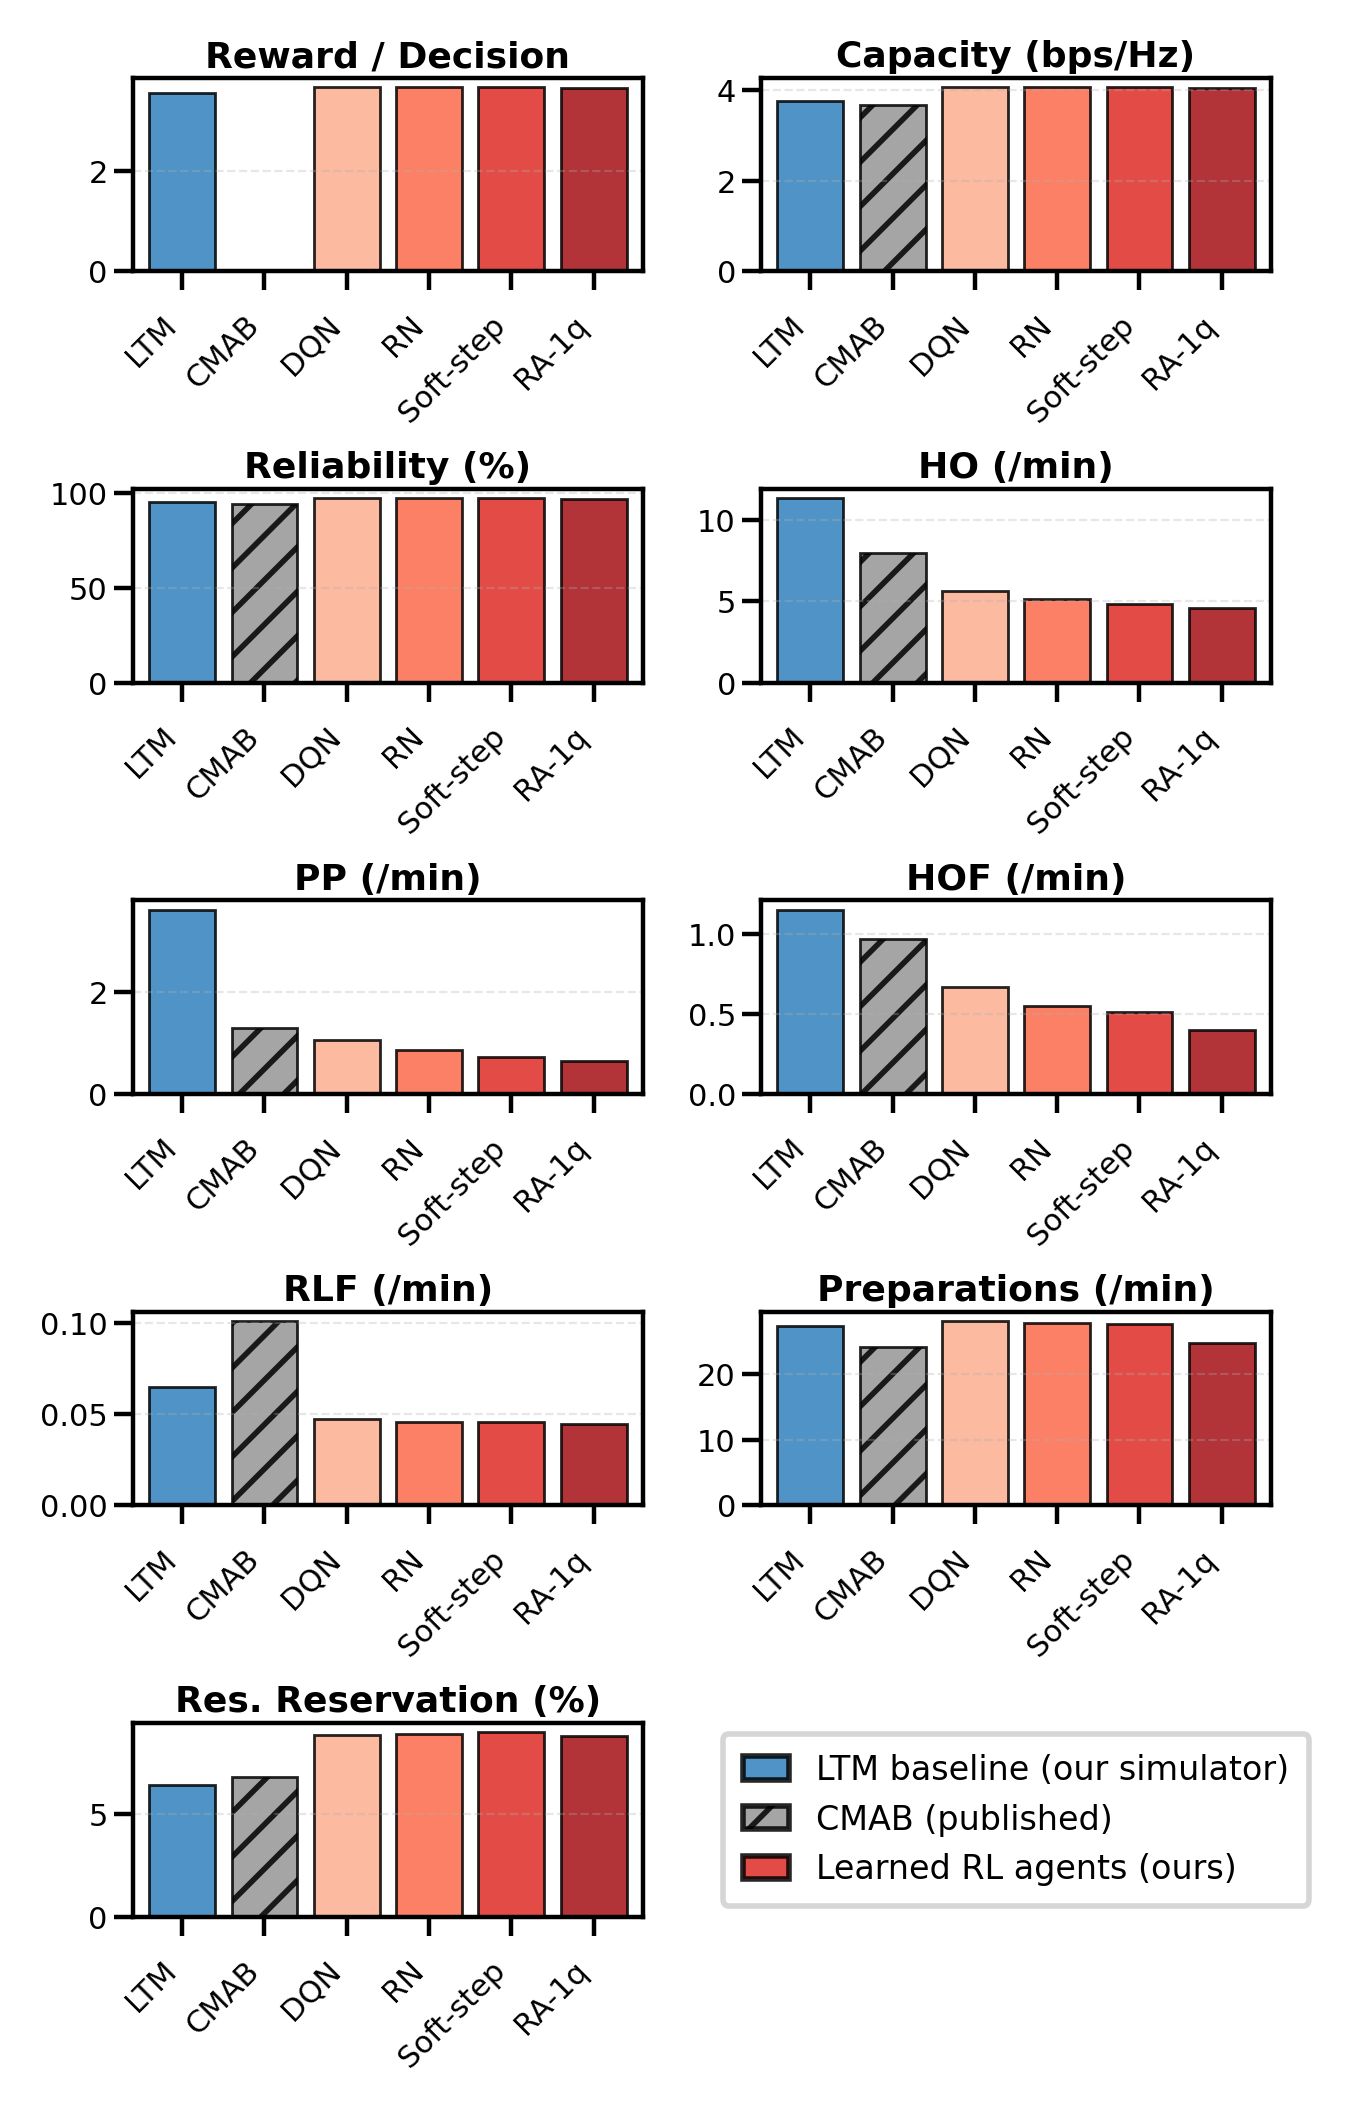
\includegraphics[width=\columnwidth]{master_bar_plots_1col.png}
\caption{Final KPI comparison on the LTM handover task (exact values in
Table~\ref{tab:final}). References first---our LTM baseline (blue)
and the published CMAB (grey, hatched, from~\cite{cmab_ho})---then the four learned
agents (red, lightest to darkest: DQN, RN, Soft-step, RA-1q). All panels start at
zero; $\downarrow$ KPIs (HO, PP, HOF, RLF, preparations, resource reservation) are
better when lower. Reward per decision is our training objective; CMAB reports none.}
\label{fig:bars}
\end{figure}


% =====================================================================
\section{Discussion, Limitations, and Future Work}
\label{sec:discussion}
\textbf{Limitations.} Several caveats bound our claims. (i)~Training and
evaluation use the \emph{same} fixed $1{,}000$-trajectory set with no held-out
split; this is the appropriate protocol for the question we ask---how well a
policy exploits a fixed propagation environment, matching the evaluation
of~\cite{cmab_ho}---but it does not measure generalization to unseen geometry.
(ii)~We study a single deployment and channel-gain dataset. (iii)~The
reward-shaping coefficients are inherited from~\cite{cmab_ho} and not re-tuned
here; the Huber threshold $\kappa$, the network width and the quantile placement, by contrast, are
swept (Sections~\ref{sec:setup},~\ref{sec:results-dist})
and have little effect on the operating point. (iv)~We explore CVaR and its spectral
(soft-step) relaxations, but not the wider space of coherent or distortion risk
measures, which may trade the KPIs off differently.

\textbf{Future work.} Several directions follow naturally. Implicit and
fully-parameterized quantile networks (IQN~\cite{iqn}, FQF~\cite{fqf}) learn the
quantile fractions themselves and would subsume the quantile-placement study.
Constrained or multi-objective formulations could bound the handover- or
radio-link-failure rate directly, rather than through the scalar reward. Our agent
also learns only the \emph{execution} decision while the candidate
\emph{preparation} stage stays fixed to the LTM heuristic; learning a risk-aware
preparation policy---not only execution---is a natural extension, as is closing the
one gap where the learned policies trail the heuristics, their higher resource
reservation, which a reservation-aware reward term could price in directly.
Finally, it remains to confirm that the distributional and quantile-placement
findings transfer to standard finite-action RL benchmarks such as the Atari~2600
suite.


% =====================================================================
\section{Conclusion}
\label{sec:conclusion}
On the LTM handover task, distributional RL delivers two separable improvements
over scalar DQN. First, the distributional learning target alone---the
risk-neutral RN agent---lowers the handover, ping-pong and failure rates and
raises capacity and reliability at equal reward per decision. Second, making the
policy risk-averse with a CVaR criterion drives the failure tails down further,
trading a small, controllable amount of reward for reliability along a monotone
risk dial with a knee near $\alpha=0.25$. The most effective realization is the
single, dedicated quantile (RA-1q): trained and acting on one tail quantile, it
attains the lowest handover, ping-pong and failure rates of any learned
agent---cutting DQN's handover-failure rate by $40\%$---at the output size and
inference cost of scalar DQN. Against our hand-tuned LTM baseline in the same
simulator it improves every user-facing and safety KPI while issuing \emph{fewer}
handovers, and it improves on the published contextual-bandit figures on the
quality KPIs; the only metric on which the heuristics lead is resource
reservation. For the lower tail that governs handover reliability, one well-placed
quantile is enough---``learn what you act on.''

% =====================================================================
\section*{Acknowledgments}
The author thanks Josep Vidal and Marga Cabrera for their mentoring and
guidance throughout this work, and Ainna Yue Moreno-Locubiche for providing the
base LTM simulation code and for help in debugging the simulator.

% =====================================================================
\begin{thebibliography}{00}
\bibitem{cmab_ho} A. Y. Moreno-Locubiche, J. Vidal, O. Mu\~{n}oz-Medina, and M. Cabrera-Bean, ``Contextual bandits and reconfigurable intelligent surfaces for predictive LTM handover decisions,'' 2025, arXiv:2512.08556.
\bibitem{c51} M. G. Bellemare, W. Dabney, and R. Munos, ``A distributional perspective on reinforcement learning,'' in \emph{Proc. ICML}, 2017.
\bibitem{qrdqn} W. Dabney, M. Rowland, M. G. Bellemare, and R. Munos, ``Distributional reinforcement learning with quantile regression,'' in \emph{Proc. AAAI}, 2018.
\bibitem{iqn} W. Dabney, G. Ostrovski, D. Silver, and R. Munos, ``Implicit quantile networks for distributional reinforcement learning,'' in \emph{Proc. ICML}, 2018.
\bibitem{fqf} D. Yang, L. Zhao, Z. Lin, T. Qin, J. Bian, and T.-Y. Liu, ``Fully parameterized quantile function for distributional reinforcement learning,'' in \emph{Proc. NeurIPS}, 2019.
\bibitem{acerbi} C. Acerbi, ``Spectral measures of risk: A coherent representation of subjective risk aversion,'' \emph{J. Banking Finance}, vol.~26, no.~7, pp.~1505--1518, 2002.
\bibitem{rockafellar} R. T. Rockafellar and S. Uryasev, ``Optimization of conditional value-at-risk,'' \emph{J. Risk}, vol.~2, pp.~21--41, 2000.
\bibitem{chow2014} Y. Chow and M. Ghavamzadeh, ``Algorithms for CVaR optimization in MDPs,'' in \emph{Proc. NeurIPS}, 2014.
\bibitem{tamar2015} A. Tamar, Y. Glassner, and S. Mannor, ``Optimizing the CVaR via sampling,'' in \emph{Proc. AAAI}, 2015.
\bibitem{dqn} V. Mnih \emph{et al.}, ``Human-level control through deep reinforcement learning,'' \emph{Nature}, vol.~518, pp.~529--533, 2015.
\bibitem{code} G. Grau Garcia, ``Distributional RL for LTM handover (source code),'' GitHub repository, 2025. [Online]. Available:\\\url{https://github.com/gerardgrau/Distributional-RL-for-LTM-Handover}
\end{thebibliography}

\end{document}
